% Runtime specifications
Models were run on a Windows 11 computer with an AMD Ryzen 5 5625U 2.3GHz processor with 16 GB of RAM\@. Gurobi version 10.0.1 was used with Python version 3.9.16. 

We aimed to compare 7 models: The pure MIP, the network model, an iterative LBBD1 (iLBBD1), LBBD1 using lazy constraints (cLBBD1), iterative LBBD2 with propagation (iLBBD2p), LBBD2 with lazy constraints and propagation (cLBBD2p) and LBBD4 with lazy constraints and propagation (cLBBD4). The pure MIP was used as a baseline.\ iLBBD1 and cLBBD1  were chosen to be used as baseline LBBD models. LBBD2 with propagation was chosen as it was one of the best performers in the original paper, we intended to use it as the main comparison to the network model and our new cut. We chose to collect results for LBBD4 only using propagation and lazy constraints as we believed this would give us the best results while adhering to the project time constraints.

We generate 5 seeded instances of data similarly to~\cite{roshanaei2017propagating}. The data is generated for 3 hospitals and 5 operating rooms over a 5 day planning horizon for varying number of patients. Unlike~\cite{roshanaei2017propagating} who generate a set of data for 3 and 5 operating rooms while only varying the surgery times in each instance, we generate each instance with entirely different data. This was believed to give results more indicative of performance on a wider variation in problem parameters. Also unlike in the original paper, where models were ran with a time limit of 7200 seconds, we set our time limit to 900 seconds due to project time constraints. At a time limit of 7200 seconds the worst case time to run all models over all 5 instances was 70 hours for only one patient size. For this same reason we only ran models with 5 available operating rooms, instead of testing both 5 and 3. We chose to use 5 operating rooms, this should have led to harder sub problems and relatively easier master problems compared to using 3 operating rooms\cite{roshanaei2017propagating}. 

There was uncertainty as to whether the models were solved to true optimality or to a relative MIP gap of $1\%$ as was done by~\cite{guo}, so we report results for both scenarios. We follow~\cite{roshanaei2017propagating} by defining the best performing model to be the most robust, that is, the one able to solve the model to optimality within the given time constraints while breaking ties by considering the fastest models averaged over solved instances.

The 7 models were solved to optimality on each of the 5 instances, the average time to solve can be seen in Table~\ref{tab:avgTimeOpt} and the average gaps can be seen in Table~\ref{tab:avgGapOpt}.

\begin{table*}
    \centering
    \caption{Average time (seconds) until solved to optimality over 5 instances. The number of instances not solved to optimality are superscripted. Non-solved instances are not included in average. **** represents that no instances solved in time.}
    \begin{tabular}{rrrrrrrr} \toprule
        $|\mathcal{P}|$ & Pure MIP & Network & iLBBD1 & cLBBD1 & iLBBD2p & cLBBD2p & cLBBD4p \\ \midrule
        20              & 16.06 &     ${****}^{(5)}$    & 1.509 &  0.8829 & 1.431 & 0.8800 & 0.7890 \\
        40              & $179.3^{(2)}$ & $268.5^{(3)}$   &  $4.429$ & $1.911^{(4)}$ & $4.503^{(1)}$ & $1.911^{(4)}$ & $1.959^{(4)}$ \\
        60 & $30.80^{(4)}$ & ${****}^{(5)}$ & $24.46^{(1)}$ & $10.73^{(4)}$ & $34.61^{(2)}$ & $21.46^{(4)}$ & $25.80^{(4)}$ \\
        80 & ${****}^{(5)}$ & ${****}^{(5)}$ & ${****}^{(5)}$ & ${****}^{(5)}$ & ${****}^{(5)}$ & ${****}^{(5)}$ & ${****}^{(5)}$ \\
        \bottomrule
    \end{tabular}
\end{table*}


We can see from Table~\ref{tab:avgTimeOpt} that all models had difficulty solving to optimality for number of patients greater than only 20. The pure MIP was the most robust across all patient sizes while the network model was the least. We can see that for sizes where LBBD models do solve an instance, they do so on average faster than the pure MIP.\@ For example, for a patient size of 20 cLBBD4p performed the best, being solved in the least time on average, with cLBBD2p being close second. For a patient size of 60, most LBBD models solved faster than the pure MIP.\@ Comparing between LBBD models, all using lazy constraints outperform those using iteration in terms of time to solve for every number of patients. The results shown in Table~\ref{tab:avgTimeOpt} suggest that none of the 7 models scale well for solving problems with sets of patients as large or larger than 60 when solving to optimality. No models were able to solve instances with 80 patients to optimality. 

\begin{table*}
    \centering
    \caption{Average gap (\%) over 5 instances after trying to solve to optimality. MIPGap is reported for pure MIP, Network and callback implementations of LBBD.\@ Gap between master problem lowerbound and best sub problem upperbound is report for iterative implementations of LBBD.}\label{tab:avgGapOpt}
    \begin{tabular}{rrrrrrrr} \toprule
        $|\mathcal{P}|$ & Pure MIP & Network & iLBBD1 & cLBBD1 & iLBBD2p & cLBBD2p & cLBBD4p \\ \midrule
        20              & 0.000 &    $0.4950$     & 0.000 &  0.000 & 0.000 & 0.000 & 0.000 \\
        40              & $0.04220$ & $0.3382 $  & $0.6252 $ & $0.3532 $ & $0.09500 $ & $0.4765 $ & $0.4948$ \\
        60 & $0.1827 $ & $0.4131 $ & $0.5514 $ & $0.2540 $ & $0.1700 $ & $0.3513 $ & $0.3273 $ \\
        80 &  $0.2630 $ &  $0.2048 $ & $0.9390$ &  $0.6000 $ & $0.2100$ & $0.4718 $ & $0.5218$ \\
        \bottomrule
    \end{tabular}
\end{table*}


Table~\ref{tab:avgGapOpt} shows that although not many instances solved to optimality, by the end of the prescribed time limit, the optimality gaps were very small. All optimality gaps had reached at least 1\% or lower. In fact, increasing the number of patients did not appear to have a large negative effect on the final optimality gaps, giving merit to the scalability of all models in term of achieving a small gap in under 15 minutes for increasing number of patients. Interestingly, nearly all gaps for number of patients greater than 20 were of the same magnitude, it seems there is some threshold that the model can reach very quickly but closing the last of the gap becomes difficult. These results gave more motivation to investigate solving to a 1\% gap.

The 7 models were solved to a 1\% gap on each of the 5 instances, the average time to solve can be seen in Table~\ref{tab:avgTimeOpt1Perc}.
%  and the average gaps can be seen in Table~\ref{tab:avgGapOpt1Perc}.

\begin{table*}
    \centering
    \caption{Average time (seconds) until solved to optimality with a 1\% gap over 5 instances. The gap used to terminate optimisation was the MIPGap for all models except for iterative LBBDs which were terminated by gap between master problem and sub problem. The number of instances not solved to optimality are superscripted. Non-solved instances are not included in average. Asterisks represent that no instances solved in time.}\label{tab:avgTimeOpt1Perc}
    \begin{tabular}{rrrrrrrr} \toprule
        $|\mathcal{P}|$ & Pure MIP & Network & iLBBD1 & cLBBD1 & iLBBD2p & cLBBD2p & cLBBD4p \\ \midrule
       20&  0.8406 & 94.56 & 0.2942 & 0.6679 & 0.6466 & 0.6335 & 0.6047 \\
       40  &5.448 & 17.52 & $28.90^{(1)}$&  58.87&  $52.35^{(1)}$ & $46.21^{(1)}$ & $6.077^{(1)}$ \\
       60 & 6.012&  29.11&  101.8 & 15.74&  $12.01^{(1)}$&  45.06 & 36.22\\
       80 & 9.716&  30.48&  34.90 & $71.66^{(1)}$&  18.79 & 62.25 & 175.4\\
       \bottomrule
    \end{tabular}
\end{table*}

% \begin{table*}
    \centering
    \caption{Average gap (\%) over 5 instances after trying to solve to optimality with a 1\% gap. MIPGap is reported for pure MIP, Network and callback implementations of LBBD.\@ Gap between master problem lowerbound and best sub problem upperbound is report for iterative implementations of LBBD.}\label{tab:avgGapOpt1Perc}
    \begin{tabular}{rrrrrrrr} \toprule
        $|\mathcal{P}|$ & Pure MIP & Network & iLBBD1 & cLBBD1 & iLBBD2p & cLBBD2p & cLBBD4p \\ \midrule
        20 & 0.9675&  0.903&     0.0 & 0.7989&      0.0 & 0.9242 & 0.9166 \\
        40&  0.9005&  0.5333&  0.3343&  0.8768&  0.6572&  0.8798&  0.8963 \\
        60&  0.7684&  0.7727&  0.2791&  0.8142&  0.7442&  0.7041&  0.9207\\
        80&  0.7875&  0.8781&  0.3236&  0.983 & 0.4335&  0.8632&  0.7431\\
        \bottomrule
    \end{tabular}
\end{table*}
 

We can see from Table~\ref{tab:avgTimeOpt1Perc} that now only going to a 1\%, most models are able to complete for most instances for number of patients up to 80. The pure MIP and the network model were the most robust across all number of patients. The least robust model across all number of patients was iLBBD2p. For 20 patients iLBBD1 solved the fastest on average. For all other number of patients the pure MIP solved the fastest. Overall, lazy constraint implementations were slightly better than there iterative counterparts.\ cLBBD2p performed better than iLBBD2p for 20, 40 and 60 patients.\ cLBBD1 performed better than iLBBD1 for 40 and 60 patients. 

The average time in the master problem and sub problem when trying to solve to a 1\% gap was plotted for different patient set sizes and can be seen in Figure~\ref{fig:MPSPtime}.

\begin{figure*}
    \centering
    \begin{subfigure}[b]{0.35\textwidth}
        \centering
        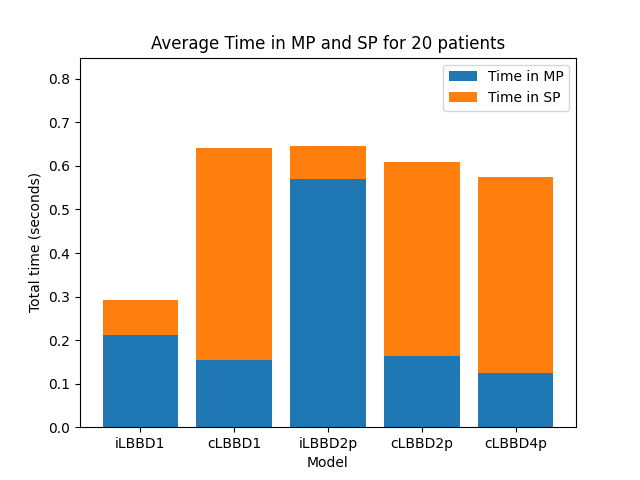
\includegraphics[width=\textwidth]{plots/(20_timeinMPSP).png}
        \caption{$|P|=20$}\label{fig:p=20}
    \end{subfigure}
    \begin{subfigure}[b]{0.35\textwidth}
        \centering
        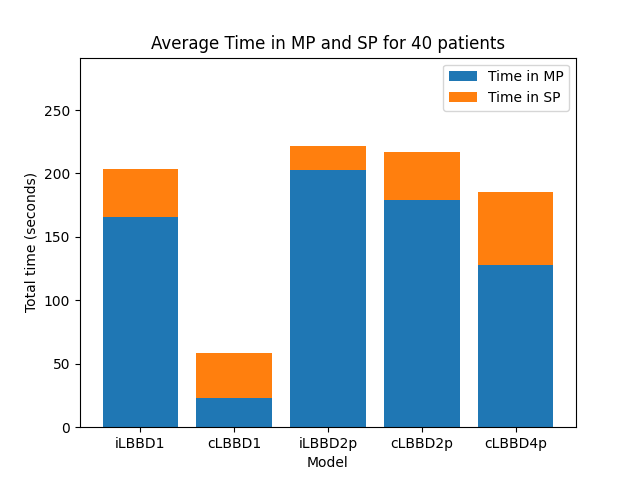
\includegraphics[width=\textwidth]{plots/(40_timeinMPSP).png}
        \caption{$|P|=40$}\label{fig:p=40}
    \end{subfigure}
    \begin{subfigure}[b]{0.35\textwidth}
        \centering
        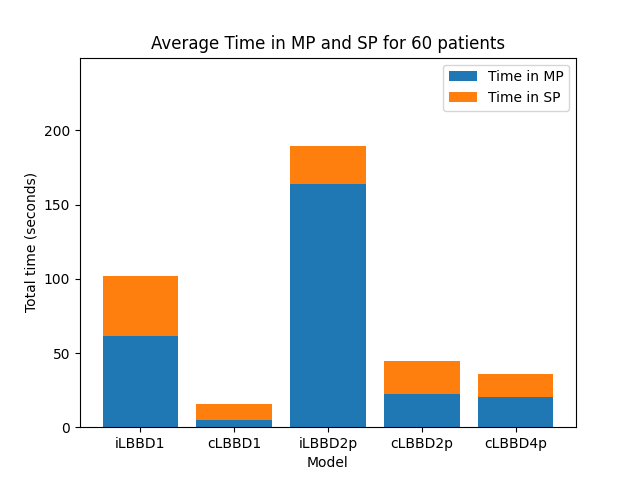
\includegraphics[width=\textwidth]{plots/(60_timeinMPSP).png}
        \caption{$|P|=60$}\label{fig:p=60}
    \end{subfigure}
    \begin{subfigure}[b]{0.35\textwidth}
        \centering
        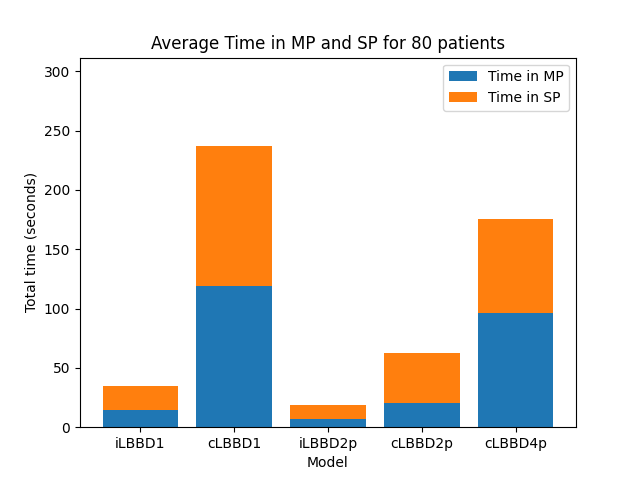
\includegraphics[width=\textwidth]{plots/(80_timeinMPSP).png}
        \caption{$|P|=80$}\label{fig:p=80}
    \end{subfigure}
    \caption{Average time in master problem (MP) and sub problem (SP) for different patient set sizes.}\label{fig:MPSPtime}
\end{figure*}

From Figure~\ref{fig:p=20} we can see that that iterative variants of LBBD spent a high proportion of their time in the master problem and the lazy constraint implementations spent a high proportion of their time in the sub problems. This is expected for the iterative implementation a large amount of time would be spent re-building the master problem branch-and-bound tree on every iteration. This is expected for the sub problem as we need to solve the sub problems for every incumbent solution, even though it was hoped to be remedied somewhat by caching of sub problems.  

Figure~\ref{fig:p=40} shows that for $|P|=40$ most variants of LBBD including lazy constraint implementations spent large portions of their time in the master problem. This provided some evidence that sub problem implementation was not the main bottleneck for this size of problem, but was in fact the highly optimized Gurobi solver. 

Across all patient set sizes shown in Figure~\ref{fig:MPSPtime} iterative versions consistently spent a high portion of their time in the master problem. Lazy constraint versions seemed to vary with regards to whether they spent more time in master problem or sub problem, this indicates that the relative difficulty of sub problems to master problems was likely highly dependent on the data and not a product of lazy constraints, this was even with using 5 operating rooms which should have influenced the problem to have easier master problems than sub problems\cite{roshanaei2017propagating}.